% % % Headers and definitions
\documentclass[10pt]{article}

\usepackage{setspace}
\usepackage{geometry}
\usepackage{fontspec} 
\usepackage{wrapfig}
\setmainfont{Times New Roman}

\doublespacing
\geometry{lmargin=1in, rmargin=0.5in, tmargin=1in, bmargin=0.75in}
\begin{document}

% Title and author
\Large{\center{\textbf{{Nick Levesque\\
April 7, 2015\\
ECE 331\\}}}}

\pagenumbering{arabic}
\large
% % % % % % % % % % % % % % %
% Introduction section
\section{Introduction}

\noindent This report describes in detail the design, testing, and validation of the RGB LED kernel module. The module takes three unsigned integers as input, and passes color values to an XMega32E5 on an external board, which drives the RGB LED with pulse-width modulation (PWM) . This module was designed so that multiple processes can open the associated device driver special file simultaneously, with locking used to limit writes to the external board to one process at a time. It is designed for use with all official models of the Raspberry Pi, up to and including the Raspberry Pi 2. 


% % % % % % % % % % % % % % %
% Design and analysis section
\section{Design}
In this section the design details, decisions, and the engineering rationale behind them are discussed.
\subsection{RGB Data}
\noindent To pass color data to the XMega, eleven bits are sent over three GPIO pins (thirty-three total bits in a sequence), with a fourth pin used as a clock. The most significant bits are sent first. In the module's initialization function, these pins are requested from the system and set as outputs with an initial value of zero. The kernel module is passed a struct containing three unsigned integers via an ioctl call. These integers contain the intensity values for red, green and blue. The duty cycle of the XMega's PWM output to each LED pin is high when the LED is dim, and low when the LED is at full brightness. Taking this into account, the module's ioctl handler runs a loop, decrementing a counter, \emph{i} from its initial value of ten until it reaches zero. In each iteration of the loop, the color values are shifted right by \emph{i}. The two's complement of this result is bitwise-ANDed with one, with the relevant GPIO pin being set high if the result is one. The ioctl handler sets the clock high, sets the pins to zero, sets the clock low, then continues looping until finished the sequence.


\subsection{Locking}
\noindent
\begin{wrapfigure}{o}{0.45\textwidth}
    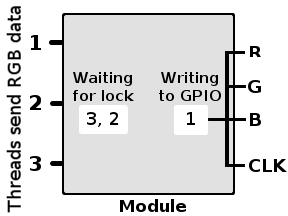
\includegraphics[width=0.45\textwidth]{figure1}
  \caption{Illustration of multi-thread handling}
\end{wrapfigure}
\noindent In order to handle multiple threads attempting to set the LED color simultaneously, only one thread is allowed to write its bit sequence at a time. Mutex locking is used to manage waiting threads. As shown in Figure 1, thread \#1 is currently writing to the GPIO pins, but thread \#2 and \#3 also want to write. Thread \#2 attempted to write before \#3, so it will acquire the lock as soon as \#1 releases it. Thread \#2 will then write its bit sequence, unlock the lock, and thread \#3 will acquire it. This prevents multiple threads from writing to GPIO pins simultaneously. The module avoids deadlock by ensuring that all paths of exit out of the locked ioctl section force the release of the lock.

\subsection{Error Checking}
\noindent Ensuring that userspace programs are returned appropriate errors when accessing the kernel module incorrectly is critical for debugging purposes, and for preventing undefined behavior. The guarantee that user input will not cause a kernel module to wreak havoc on a system is important.
\newline
\noindent Appropriate errors are returned for all cases where the user does something wrong. User input passed via ioctl is checked for validity, and invalid pointers passed via ioctl are caught. User code attempting to open the device special file as anything besides write-only is returned an "operation not supported" error. Also, user code which uses a read-write or read-only ioctl call is returned an "invalid ioctl command" error.

% % % % % % % % % % % % % % %
% Testing / Validation
\section{Testing and Validation}
The included test suite thoroughly tests the performance and capability of the kernel module. It is located in \emph{test/}. 
\subsection{Autotest} The \emph{autotest} program runs through twenty test cases, which are documented in \emph{testcases.txt}. Each test compares an expected output to the actual output from the module. If both are equal, the test passes. Additionally, \emph{autotest} tries five valid attempts to set the RGB LED color. Whether the set colors are correct or not must be determined visually, because \emph{autotest} does not have human eyes.

\subsection{Threadtest}
The second component of the test suite, \emph{threadtest}, tests the capability of the kernel module to handle access by multiple threads. This C program fades the LED from red to green to blue by looping through values 0-2047 for each color, and writing each color value via ioctl as a separate child process. Each child process must wait its turn for the lock. The LED fades smoothly, indicating that locking is working correctly and multiple processes are not allowed to send bits over GPIO pins simultaneously.

\subsection{Client}
A rudimentary client is included in the \emph{client/} directory. Testing specific colors can be done by passing three integers between 0 and 2047 as arguments to the client.

% % % % % % % % % % % % % % %		
% Results / Conclusion
\section{Results and Conclusion}
\noindent The resulting kernel module offers a 60ms improvement (as measured by the "real" result from the \emph{time} utility) in performance over an RGB LED client, previously developed as a homework assignment, which uses the bcm2835.h library.
\newline

\noindent The final result of this project is an operational kernel module which sets the color of an external RGB LED based on three unsigned integers passed by a user. It prevents race conditions through locking, and avoids deadlock. The module handles errors correctly, and passes errors to the user program when appropriate. It passes all tests described in the \emph{Testing and Validation} section. 


\end{document}
